\documentclass[11pt,a4paper]{jsarticle}
\usepackage{amsmath,amssymb}
\usepackage{amsthm}
\usepackage{ascmac}
\usepackage{bm}
\usepackage[dvipdfmx]{graphicx}	% required for `\includegraphics' (yatex added)
\usepackage{setspace}           % required for `\doublespace'
\usepackage{tikz}
\usepackage{tikz-cd}
\usetikzlibrary{angles, positioning, shapes, arrows.meta, decorations.pathmorphing}
%\usetikzlibrary{intersections, calc, arrows, positioning, arrows.meta}
\usepackage{tcolorbox}  % 定理環境の装飾
\tcbuselibrary{skins, breakable, theorems}
\usepackage{xcolor}
\usepackage{natbib}
\usepackage{pxrubrica}
\usepackage[margin=30truemm, left=40truemm, right=40truemm]{geometry}
\usepackage{thmbox}     % required for theorem environment with side bar
%
\setlength{\parskip}{3mm} %段落間にスペースを入れる


% \pagestyle{myheadings}
% \markright{\footnotesize \sf 2022秋期「哲学者のための数学」授業資料(大塚淳) \ \ 配布禁止}


\theoremstyle{definition}
\newtheorem[S]{exercise}{練習問題}[section]
\newtheorem[S]{example}{事例}[section]
\newtheorem[S]{fact}{事実}[section]
\newtheorem[S]{attn}{注意}[section]
\newtheorem[S]{develop}{発展}[section]
\renewcommand{\theattn}{}

\newtcbtheorem[auto counter, number within=section]{rei}{事例}{
    breakable,
    coltitle=black,
    fonttitle=\bfseries,
    enhanced, colback=white, frame hidden, borderline west = {0.5pt}{5pt}{black},
%    number freestyle={\noexpand\thesection.\noexpand\arabic{\tcbcounter}}
}{rei}

\newtcbtheorem[auto counter, number within=section]{prop}{命題}{
    breakable,
    coltitle=black,
    fonttitle=\bfseries,
    enhanced, colback=white, frame hidden, borderline west = {0.5pt}{5pt}{black},
%    number freestyle={\noexpand\thesection.\noexpand\arabic{\tcbcounter}}
}{prop}

\newtcbtheorem[number within=section]{renshu}{練習問題}{
    breakable,
    coltitle=black,
    fonttitle=\bfseries,
    enhanced, colback=white, frame hidden, borderline west = {0.5pt}{5pt}{black}
}{renshu}


\newtcbtheorem[number within=section]{hatten}{発展}{
    breakable,
    coltitle=black,
    fonttitle=\bfseries,
    enhanced, colback=white, frame hidden, borderline west = {0.5pt}{5pt}{black}
}{renshu}


\newtcbtheorem[number within=section]{dfn}{定義}{
    fonttitle=\bfseries,
    enhanced, colback=white
}{dfn}


% Bold face capital letters:
\newcommand{\bfzero}{\boldsymbol{0}}
\newcommand{\bfone}{\boldsymbol{1}}
\newcommand{\bfA}{\boldsymbol{A}}
\newcommand{\bfB}{\boldsymbol{B}}
\newcommand{\bfC}{\boldsymbol{C}}
\newcommand{\bfD}{\boldsymbol{D}}
\newcommand{\bfE}{\boldsymbol{E}}
\newcommand{\bfF}{\boldsymbol{F}}
\newcommand{\bfG}{\boldsymbol{G}}
\newcommand{\bfH}{\boldsymbol{H}}
\newcommand{\bfI}{\boldsymbol{I}}
\newcommand{\bfJ}{\boldsymbol{J}}
\newcommand{\bfK}{\boldsymbol{K}}
\newcommand{\bfL}{\boldsymbol{L}}
\newcommand{\bfM}{\boldsymbol{M}}
\newcommand{\bfN}{\boldsymbol{N}}
\newcommand{\bfO}{\boldsymbol{O}}
\newcommand{\bfP}{\boldsymbol{P}}
\newcommand{\bfQ}{\boldsymbol{Q}}
\newcommand{\bfR}{\boldsymbol{R}}
\newcommand{\bfS}{\boldsymbol{S}}
\newcommand{\bfT}{\boldsymbol{T}}
\newcommand{\bfU}{\boldsymbol{U}}
\newcommand{\bfV}{\boldsymbol{V}}
\newcommand{\bfW}{\boldsymbol{W}}
\newcommand{\bfX}{\boldsymbol{X}}
\newcommand{\bfY}{\boldsymbol{Y}}
\newcommand{\bfZ}{\boldsymbol{Z}}

\newcommand{\bfa}{\boldsymbol{a}}
\newcommand{\bfb}{\boldsymbol{b}}
\newcommand{\bfc}{\boldsymbol{c}}
\newcommand{\bfd}{\boldsymbol{d}}
\newcommand{\bfe}{\boldsymbol{e}}
\newcommand{\bff}{\boldsymbol{f}}
\newcommand{\bfk}{\boldsymbol{k}}
\newcommand{\bfm}{\boldsymbol{m}}
\newcommand{\bfn}{\boldsymbol{n}}
\newcommand{\bfo}{\boldsymbol{o}}
\newcommand{\bfp}{\boldsymbol{p}}
\newcommand{\bfq}{\boldsymbol{q}}
\newcommand{\bfr}{\boldsymbol{r}}
\newcommand{\bfs}{\boldsymbol{s}}
\newcommand{\bft}{\boldsymbol{t}}
\newcommand{\bfu}{\boldsymbol{u}}
\newcommand{\bfv}{\boldsymbol{v}}
\newcommand{\bfw}{\boldsymbol{w}}
\newcommand{\bfx}{\boldsymbol{x}}
\newcommand{\bfy}{\boldsymbol{y}}
\newcommand{\bfz}{\boldsymbol{z}}



% BB (???) capital letters:
\newcommand{\bbA}{\mathbb{A}}
\newcommand{\bbB}{\mathbb{B}}
\newcommand{\bbC}{\mathbb{C}}
\newcommand{\bbD}{\mathbb{D}}
\newcommand{\bbE}{\mathbb{E}}
\newcommand{\bbF}{\mathbb{F}}
\newcommand{\bbG}{\mathbb{G}}
\newcommand{\bbI}{\mathbb{I}}
\newcommand{\bbN}{\mathbb{N}}
\newcommand{\bbP}{\mathbb{P}}
\newcommand{\bbQ}{\mathbb{Q}}
\newcommand{\bbR}{\mathbb{R}}
\newcommand{\bbU}{\mathbb{U}}
\newcommand{\bbV}{\mathbb{V}}
\newcommand{\bbX}{\mathbb{X}}
\newcommand{\bbY}{\mathbb{Y}}
\newcommand{\bbZ}{\mathbb{Z}}
\newcommand{\bbone}{{\ifmmode\mathrm{1\!l}\else\mbox{\(\mathrm{1\!l}\)}\fi}}


% Caligraphic math capital letters:
\newcommand{\mcalA}{\mathcal{A}}
\newcommand{\mcalB}{\mathcal{B}}
\newcommand{\mcalC}{\mathcal{C}}
\newcommand{\mcalD}{\mathcal{D}}
\newcommand{\mcalE}{\mathcal{E}}
\newcommand{\mcalF}{\mathcal{F}}
\newcommand{\mcalG}{\mathcal{G}}
\newcommand{\mcalH}{\mathcal{H}}
\newcommand{\mcalI}{\mathcal{I}}
\newcommand{\mcalJ}{\mathcal{J}}
\newcommand{\mcalK}{\mathcal{K}}
\newcommand{\mcalL}{\mathcal{L}}
\newcommand{\mcalM}{\mathcal{M}}
\newcommand{\mcalN}{\mathcal{N}}
\newcommand{\mcalO}{\mathcal{O}}
\newcommand{\mcalP}{\mathcal{P}}
\newcommand{\mcalQ}{\mathcal{Q}}
\newcommand{\mcalS}{\mathcal{S}}
\newcommand{\mcalT}{\mathcal{T}}
\newcommand{\mcalU}{\mathcal{U}}
\newcommand{\mcalV}{\mathcal{V}}
\newcommand{\mcalX}{\mathcal{X}}
\newcommand{\mcalY}{\mathcal{Y}}
\newcommand{\mcalZ}{\mathcal{Z}}

% Graph nodes notations:
\newcommand{\PA}{\mathit{PA}}
\newcommand{\bfPA}{\mathbf{PA}}
\newcommand{\CH}{\mathit{CH}}
\newcommand{\bfCH}{\mathbf{CH}}
\newcommand{\DS}{\mathit{DS}}
\newcommand{\bfDS}{\mathbf{DS}}
\newcommand{\ND}{\mathit{ND}}
\newcommand{\bfND}{\mathbf{ND}}
\newcommand{\AN}{\mathit{an}}
\newcommand{\bfAN}{\mathbf{an}}
\newcommand{\pa}{\mathit{pa}}
\newcommand{\bfpa}{\mathbf{pa}}
\newcommand{\ch}{\mathit{ch}}
\newcommand{\bfch}{\mathbf{ch}}
\newcommand{\ds}{\mathit{ds}}
\newcommand{\bfds}{\mathbf{ds}}
\newcommand{\nd}{\mathit{nd}}
\newcommand{\bfnd}{\mathbf{nd}}
\newcommand{\an}{\mathit{an}}
\newcommand{\bfan}{\mathbf{an}}



\DeclareMathOperator*{\argmax}{arg\,max}
\DeclareMathOperator*{\argmin}{arg\,min}
\DeclareMathOperator*{\argsup}{arg\,sup}
\DeclareMathOperator*{\arginf}{arg\,inf}
\DeclareMathOperator{\erfc}{erfc}
\DeclareMathOperator{\diag}{diag}
\DeclareMathOperator{\cum}{cum}
\DeclareMathOperator{\sgn}{sgn}
\DeclareMathOperator{\tr}{tr}
\DeclareMathOperator{\spn}{span}
\DeclareMathOperator{\adj}{adj}
\DeclareMathOperator{\E}{\mathbb{E}}
\DeclareMathOperator{\var}{Var}
\DeclareMathOperator{\cov}{Cov}
\DeclareMathOperator{\corr}{corr}
\DeclareMathOperator{\sech}{sech}
\DeclareMathOperator{\sinc}{sinc}
\DeclareMathOperator*{\lms}{l.i.m.\,}
\newcommand{\varop}[1]{\var\left[{#1}\right]}
\newcommand{\covop}[2]{\cov\left({#1},{#2}\right)}
\newcommand{\T}{^\textrm{T}}
\newcommand\indep{\protect\mathpalette{\protect\independenT}{\perp}}
\def\independenT#1#2{\mathrel{\rlap{$#1#2$}\mkern2mu{#1#2}}}

\newcommand{\bfalpha}{\boldsymbol{\alpha}}
\newcommand{\bfbeta} {\boldsymbol{\beta}}
\newcommand{\bfgamma}{\boldsymbol{\gamma}}
\newcommand{\bfeta}  {\boldsymbol{\eta}}
\newcommand{\bftheta}{\boldsymbol{\theta}}
\newcommand{\bflambda}   {\boldsymbol{\lambda}}
\newcommand{\bfmu}   {\boldsymbol{\mu}}
\newcommand{\bfnu}   {\boldsymbol{\nu}}
\newcommand{\bfxi}   {\boldsymbol{\xi}}
\newcommand{\bfpsi}  {\boldsymbol{\psi}}
\newcommand{\bfphi}   {\boldsymbol{\phi}}
\newcommand{\bfrho}   {\boldsymbol{\rho}}
\newcommand{\bfvarepsilon}{\boldsymbol{\varepsilon}}
%\newcommand{\qed}{{qed}}
%\newcommand{\eqalignno}[1]{\begin{array}{ccccccc}#1\end{array}}

\newcommand{\bfGamma}{\boldsymbol{\Gamma}}
\newcommand{\bfTheta}{\boldsymbol{\Theta}}
\newcommand{\bfLambda}   {\boldsymbol{\Lambda}}
\newcommand{\bfPsi}  {\boldsymbol{\Psi}}
\newcommand{\bfPhi}   {\boldsymbol{\Phi}}
\newcommand{\bfSigma}  {\boldsymbol{\Sigma}}
\newcommand{\bfOmega}  {\boldsymbol{\Omega}}


% DISTRIBUTIOoNS: 
\newcommand{\normal}{\mathcal{N}}
\newcommand{\binomial}{\mathcal{B}}
\newcommand{\multinomial}{\mathcal{M}}
\newcommand{\exponential}{\mathcal{E}}
\newcommand{\geometric}{\mathcal{G}}
\newcommand{\poisson}{\mbox{Poisson}}
\newcommand{\uniform}{\mbox{Uniform}}

% Logic
\newcommand{\true}{\texttt{true}}
\newcommand{\false}{\texttt{false}}


%PSTricks (commande for latent nodes)
\newcommand{\lnode}[4]{ \cnode(#1){#2}{#3}\rput(#1){\footnotesize#4} }

% KEEPING TRACK OF WORK
\newcommand{\todo}[1]
{
{\color{red}{
[TODO: #1]}}
\addcontentsline{toc}{subsection}{TO DO: #1}
}

\newcommand{\fixme}[1]{{\color{red}{#1}}}

\newenvironment{answer}[1]
{\par \color{blue}{#1}}
{}


\newcommand{\note}[2]
{
{\color{red}{
[#1: #2]}}
}




\makeatletter
% define \citepos for posesive citation (e.g. Otsuka's (2015))
\DeclareRobustCommand\citepos
  {\begingroup
   \let\NAT@nmfmt\NAT@posfmt% ...except with a different name format
   \NAT@swafalse\let\NAT@ctype\z@\NAT@partrue
   \@ifstar{\NAT@fulltrue\NAT@citetp}{\NAT@fullfalse\NAT@citetp}}

\let\NAT@orig@nmfmt\NAT@nmfmt
\def\NAT@posfmt#1{\NAT@orig@nmfmt{#1's}}
\makeatother




% Code for drawing color circle used in topology (pathconnectedness)
\usepackage{xparse}
\ExplSyntaxOn

\keys_define:nn { colour_transition_circle } {
    inner   .fp_set:N   = \l__inner_radius,
    inner   .initial:n  = {2},
    outer   .fp_set:N   = \l__outer_radius,
    outer   .initial:n  = {3},
    angle   .fp_set:N   = \l__start_angle,
    angle   .initial:n  = {0}
}

\NewDocumentCommand \ColourTransitionCircle { O{} m } {
\group_begin:
    \keys_set:nn { colour_transition_circle } {#1}
    \clist_clear:N \l_tmpa_clist
    \clist_map_inline:nn {#2} {
        \clist_put_right:Nn \l_tmpa_clist {##1}
        %\clist_put_right:Nn \l_tmpa_clist {##1}
    }
    \exp_args:Nx \col_trans_circ:n \l_tmpa_clist
\group_end:
}

\cs_new_protected:Npn \col_trans_circ:n #1 {
    \int_step_inline:nnnn {1} {1} {\clist_count:n {#1} - 1} {
        \path[top~color=\clist_item:nn {#1} {##1}, bottom~color=\clist_item:nn {#1} {##1+1}, shading~angle={270-(180-360/\clist_count:n {#1})/2+(##1-1)*360/\clist_count:n {#1}+\fp_use:N \l__start_angle}] ({\fp_use:N \l__inner_radius*cos((##1-1)*360/\clist_count:n {#1}+\fp_use:N \l__start_angle)},{\fp_use:N \l__inner_radius*sin((##1-1)*360/\clist_count:n {#1}+\fp_use:N \l__start_angle)}) arc[radius = \fp_use:N \l__inner_radius, start~angle={(##1-1)*360/\clist_count:n {#1}+\fp_use:N \l__start_angle}, delta~angle=360/\clist_count:n {#1}] -- ({\fp_use:N \l__outer_radius*cos(##1*360/\clist_count:n {#1}+\fp_use:N \l__start_angle)},{\fp_use:N \l__outer_radius*sin(##1*360/\clist_count:n {#1}+\fp_use:N \l__start_angle)}) arc[radius = \fp_use:N \l__outer_radius, start~angle={##1*360/\clist_count:n {#1}+\fp_use:N \l__start_angle}, delta~angle=-360/\clist_count:n {#1}] -- cycle;
    }
    \path[top~color=\clist_item:nn {#1} {\clist_count:n {#1}}, bottom~color=\clist_item:nn {#1} {1}, shading~angle={180-180/\clist_count:n {#1}+\fp_use:N \l__start_angle}]({\fp_use:N \l__inner_radius*cos((\clist_count:n {#1}-1)*360/\clist_count:n {#1}+\fp_use:N \l__start_angle)},{\fp_use:N \l__inner_radius*sin((\clist_count:n {#1}-1)*360/\clist_count:n {#1}+\fp_use:N \l__start_angle)}) arc[radius = \fp_use:N \l__inner_radius, start~angle={(\clist_count:n {#1}-1)*360/\clist_count:n {#1}+\fp_use:N \l__start_angle}, delta~angle=360/\clist_count:n {#1}] -- ({\fp_use:N \l__outer_radius*cos(\clist_count:n {#1}*360/\clist_count:n {#1}+\fp_use:N \l__start_angle)},{\fp_use:N \l__outer_radius*sin(\clist_count:n {#1}*360/\clist_count:n {#1}+\fp_use:N \l__start_angle)}) arc[radius = \fp_use:N \l__outer_radius, start~angle={\clist_count:n {#1}*360/\clist_count:n {#1}+\fp_use:N \l__start_angle}, delta~angle=-360/\clist_count:n {#1}] -- cycle;
}

\ExplSyntaxOff

\begin{document}


\title{2. 関係と関数}
\author{2022秋期「哲学者のための数学」授業資料(大塚淳)}
\date{ver. \today}
\maketitle

\section{関係}
1章では,(適用基準が明確な)述語が部分集合と対応することを見た.
ただしここでの「述語」とは,「歌手である」や「偶数である」といったように,主語のみを空欄とする一項述語であった.
では「〜は...を愛する」や「〜は...で割り切れる」といったような二項述語ないし\emph{関係}(relation)は何に対応するだろうか?
これらはデカルト積の部分集合に対応する.

これを例で考えるため,$A := \{\text{Alice, Bob, Chris}\}$を人の集合,$B := \{ \text{清水寺, 金閣寺, 銀閣寺}\}$を寺社仏閣の集合として,誰がどこを訪れたことがあるかを示す表を作ってみよう.

\begin{table}[h]
\centering
\begin{tabular}{cccc} \hline
  & Alice & Bob & Chris \\ \hline 
清水寺 & \checkmark & & \checkmark \\
金閣寺 & & \checkmark &  \\
銀閣寺 & \checkmark  & \checkmark & \\ \hline
\end{tabular} 
\end{table}
この表はそのまま,$A \times B$のデカルト積を表しており,チェックマークがついているところはその部分集合を構成していると考えることができる.
なので「〜は...に行ったことがある」という二項関係は,この部分集合$R \in A \times B$と考えることができる.
具体的には
\[
 R := \{ (\text{Alice, 清水寺}), (\text{Alice, 銀閣寺}), (\text{Bob, 金閣寺}), (\text{Bob, 銀閣寺}), (\text{Chris, 清水寺}) \}
\]
であり,内包的には
\[
 R := \{ (x,y) \in A \times B| x \text{は} y \text{に行ったことがある}\}
\]
となる.「Bobは銀閣寺に行ったことがある」という事実は$(\text{Bob, 銀閣寺}) \in R$によって表される.
ちなみに$a$が$b$に対し$R$という関係を持つ,とわざわざ書くのは長いので,短く$aRb$と表すことにする.
また関係$R$に対応する部分集合を,$R$のグラフとよぶこともある.

また自然数について「〜は...以下である」という関係$\leq$は,
\[
 L := \{ (x,y) \in \bbN \times \bbN | x \leq y \}
\]
で表すことができる.例えば$(2, 5) \in L, (100, 84) \not\in L$である.

同様の仕方で,三項以上の関係も定義できる.一般に$n$関係は($n$-ary relatiohship)は$n$項積$S_1 \times \cdots \times S_n$の部分集合である.

\begin{exercise}
自然数について,「〜は...で割り切れる」という関係を内包的に定義せよ.
\end{exercise}


\section{関係の種類}
\label{sec:relation_kinds}
関係それ自体は単に積集合の部分集合に過ぎない.
しかし関係には様々な性質を持つものがあり,これは部分集合のあり方に何らかの構造的制約を課すことに対応する.
ここでは特に,一つの集合$A$を定め,そのデカルト積の中での関係$R \subset A \times A$を考えることにしよう.

すべての対象が自分自身と$R$という関係を持つとき,$R$は\emph{反射的}(reflexive)であると言われる.つまり
\[
 \forall x \in A ( (x,x) \in R )
\]
が成立する.
これは$A \times A$の表で考えると,対角線上にすべてチェックマークがついているということである.
逆にいかなる$x$についても$(x, x) \not\in R$のとき,$R$は非反射的といわれる.

$R$が\emph{対称的}(symmetric)であるとは,$xRy$ならば必ず$yRx$であるとき,つまり
\[
 \forall x, y \in A ( (x,y) \in R \Rightarrow (y,x) \in R)
\]
が成立するときである.
$A \times A$の表では,チェックマークの分布が対角線を折り目として線対称であることである.

逆に,$xRy$であれば必ず$\neg yRx$であるとき,つまり
\[
 \forall x, y \in A ( (x,y) \in R \Rightarrow (y,x) \not\in R)
\]
のとき,$R$は\emph{非対称的}(asymmetric)だといわれる.
このとき,線対称となる箇所$(x,y), (y,x)$のどちらかは必ず空欄である(両方空欄でも問題ない).
しかし対角線はすべて空欄にならなければならない.
なぜなら$(x,x) \in R$であればその前後を入れ替えたものも$R$に入ってしまうからである.
つまり非対称的な関係は非反射的である.

ややこしいが,非対称性と\emph{反対称性}(anti-symmetric)を混同しないように.
$R$が反対称であるとは,$xRy$かつ$yRx$なら$x=y$であること,つまり
\[
 \forall x, y \in A ( ((x,y) \in R \wedge  (y,x) \in R) \Rightarrow x=y).
\]
反対称的な表は対角線以外では非対称的な表と同じだが,対角線上にチェックマークが入っていてもよい,というところが異なる.
つまり反対称的な関係は非対象的だが,逆は必ずしもそうではない(反対象性は非反射性を含意しないため).

最後に,関係が\emph{推移的}(transitive)であるとは,$aRb, bRc$なら$aRc$であること,つまり
\[
 \forall x, y, z \in A ((x,y) \in R \wedge (y,z) \in R \Rightarrow (x,z) \in R)
\]
が成り立つことである.

\begin{exercise}
 $=, <, \leq$ について,それぞれ反射的/対称的/反対称的/推移的であるかどうか調べよ.
\end{exercise}

\begin{exercise}
 身近な関係性で,反射性/対称性/推移性を満たすものをそれぞれ挙げよ.
\end{exercise}


\section{同値関係と同値類}
反射的,対称的かつ推移的な関係を\emph{同値関係}(equivalence relation)という.
「(〜と...は)同じ年齢である」,「地続きである」などは同値関係の例である.
$R$が同値関係であるとき,$aRb$を特に$a\sim_R b$ないし誤解の恐れがないときは$a \sim b$と書くことがある.
このとき$a,b$は$R$に関して同値であるといわれる.

\begin{exercise}
 身近な同値関係を挙げ,それが反射性,対称性,推移性を満たすことを確認せよ.
\end{exercise}

同値関係が一つ与えられると,それによって集合の中身を類別することができる.
例として,$A$を都道府県からなる集合と,「地続きである」という同値関係$R$を考えてみよう.\footnote{なおここで「2つの県が地続きである」とは,一方の県のどこか一部から他方の県のどこか一部に陸上を歩いて到達できる,ということだとする.}
このとき,ある県$a$と地続きである県全体の集合を$[a]_R$あるいは略して$[a]$で表す.すなわち
\[
 [a] = \{x \in A | aRx\}.
\]
これを同値関係$R$による$a$の\emph{同値類}(equivalence class)あるいは\emph{類}とよぶ.
同値類は以下の性質を持つ:
\begin{align}
[a] \cap [b] \neq \emptyset & \iff [x] = [y] \\
\bigcup_{x \in A} [x] & = A
\end{align}
(1)は,もし2つの同値類が共通部分を持つならそれらは完全に等しい,逆に言えば異なる同値類は互いにオーバーラップしない,ということをいっている.
(2)は,$A$の各元の同値類をすべて合わせるともとの集合$A$と等しくなる,ということをいっている.
これは合わせて,$A$という集合は同値類によって\emph{分割}(partition)されるということを意味する.
一つ一つの同値類は,そのように分割された集合の「区画」を表す.
そうした同値類/区画の集合(つまり部分集合の集合)を$A$の$R$による\emph{商集合}とよび,$A/R$で表す.

\begin{exercise}
 $A, R$を上の例の通りとした場合,$A/R$は何個の元をもつか.
\end{exercise}

同値関係の数だけ,同値類がある.
例えば上の例で$S$を「同じ文字数である」という同値関係にした場合,$A$はまた違ったように分割される.

\begin{exercise}
「同じ漢字を持つ」という関係で$A$を同値類に分割することはできるだろうか.
%できない.推移的でないため.山口/岡山/福岡
\end{exercise}

\begin{example}
哲学において同値類は非常に重要な役割を持つ.
というのもそれは個物(トークン)の関係性からタイプや抽象的性質を作り出すことを可能にするからだ.
例えば次のような同値類を考えてみよ
\[
 [x] = \{ y | y \text{は} x \text{と同じ色である}\}
\]
これによって「同色である」という個物間の関係から,「色」という同値類が得られている.
また
\[
 [x] = \{ y | y \text{は} x \text{と並行である}\}
\]
によって「方向」という概念が得られる.
ここからわかるように,抽象というものの第一歩は同値類を作ることだといえる.
\end{example}


\begin{example}
 あるものと別のものが時空的に関係しているとき,それらは\emph{世界メイト}(world-mate)であると呼ばれる(D. Lewis).
 世界メイトが同値関係であることを確認せよ.
 またそれによって得られる同値類はなんだろうか.\footnote{ルイスについては,野上志学『デイヴィッド・ルイスの哲学』(青土社)を参照のこと.}
\end{example}


\begin{example}
 現在の生物学において主要な種概念である\emph{生物学的種概念}によれば,ある個体$a$と$b$が同じ種であるのは,両者が繁殖可能であるとき,そのときに限るとされる.これは同値類による分類だとみなしてよいだろうか.もし問題があるとしたら,それはなんだろうか.
\end{example}
% 生物学的種概念



\section{関数}
以下では関係の中でも非常に重要な,\emph{関数}(functions)を取り上げる.
集合$X$から$Y$への関数ないし\emph{写像}(mapping)とは,$X$の各要素$x$に対して必ず一つの要素$y$を対応させるような関係である.
これを
\[
 f : X \to Y
\]
と書く.
$X$を横,$Y$を縦に並べた表(グラフ)で関数を考えると,各列が必ず一個だけチェックマークを含んでいることになる.
$f$が要素$x \in X$に対して$y \in Y$を対応させることを,$f(x)=y$あるいは$f::x \mapsto y$と書いたりする.
関数の送り元(今の場合$X$)を定義域(domain),送り先を値域(codomain)とよぶ.

% \begin{exercise}
%  関数を内包的に定義してみよ.(ヒント:関係なので積集合の部分集合$\{ (x,y) \in X \times Y | \dots \}$という形になる.「$\dots$」のところには(1)すべての$x \in X$に対してその関係を満たすような$y \in Y$が存在する,(2)そのような$y$は一意である,つまりもし$x$に対し2つの$y, y'$が関係を満たすなら,$y=y'$である,という条件を入れればよい.)
% \end{exercise}

例えば「〜は...国で生まれた」という関係は,人の集合から国の集合への関数になる.
\begin{table}[h]
\centering
\begin{tabular}{ccccc} \hline
  & Alice & Bob & Chris & Dave \\ \hline 
日本 &  & \checkmark &  & \\
アメリカ & \checkmark &  &  & \checkmark \\
フランス &   &  & \checkmark & \\ \hline
\end{tabular} 
\end{table}

この関数は,それぞれの人に対し一つ,そして一つだけ出生地を割り当てている.
関数というと,例えば$y = x^3-2x$のようなものを思い浮かべるかもしれない:
\begin{figure}[h]
\centering
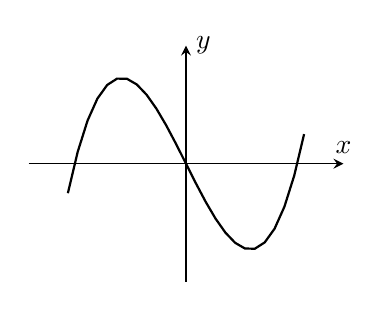
\begin{tikzpicture}[scale=1]
\draw[->,>=stealth,semithick](-2,0)--(2,0)node[above]{$x$};%x軸
\draw[->,>=stealth,semithick](0,-1.5)--(0,1.5)node[right]{$y$};%y軸
\draw[thick,domain=-1.5:1.5] plot(\x,{pow(\x,3)-2*\x});
\end{tikzpicture} 
\end{figure}

実際これは,$X, Y$を実数の集合$\bbR$としたときの関数$f:X \to Y$になっている.
グラフは各$x \in X$に対して唯一の$f(x) \in Y$を割り当てているし,また上の曲線は$\bbR \times \bbR$の部分集合になっていることを確認しよう.


\begin{develop}
ただ2つの元からなる集合$\mathbf{2} := \{0, 1\}$を考える.
$X$を任意の集合とし,関数$f:X \to \mathbf{2}$を考えると,この関数$f$は各元$x \in X$に対し0か1を割り当てることによって,$X$の部分集合$A \subset X$と同一視できる.
なぜなら,$f(x)=0$ならこの部分集合に入れ,$f(x)=1$なら入れない,というように,$f$は$A$の選択基準を与えるからだ.
こうした$f$は特性関数(characteristic function)と呼ばれ,$X$からの特性関数全体の集合を$\mathbf{2}^X$と書く,つまり
\[
 \mathbf{2}^X := \{ f|f:X \to \mathbf{2}\}.
\]
一般に,$X$からの特性関数を一つ決めると$X$の部分集合が一つ定まり,逆もまたしかり.
よって,$\mathbf{2}^X$と$\mcalP(X)$は同一視できる.
\end{develop}


\section{写像の合成}
2つの関数$f:X \to Y, g:Y \to Z$の値域と定義域が一致している場合,この2つを連結して関数$g \circ f:X \to Z$をつくることができる.この関数を$f$と$g$の\emph{合成写像}(composition)とよぶ.
具体的に合成写像$g \circ f$は,$x \in X$に対して$g(f(x)) \in Z$を対応させる.
つまり$f$で写した元をさらに$g$で写す.
$f$の後に$g$を適用するのに,$g \circ f$と書くのは一見逆な気がするが,この記法は$g(f(x))$という書き方に合わせてある.

写像の合成するとき,順序は関係ない.
つまり任意の写像$f:W \to X, g:X \to Y, h:Y \to Z$があったとき,$(h \circ g) \circ f = h \circ (g \circ f)$が成り立つ.
つまり$h$と$g$を先に合成したものと$f$を合成しても,$g$と$f$を合成したものに$h$を合成しても,同じ$W$から$Z$への写像ができる.
これを,写像の合成は\emph{結合的}(associative)である,あるは結合法則を満たす,という.

\begin{exercise}
上で見た関数$y = f(x) = x^3 -2x$は$\bbR$からそれ自身への関数であり,よって合成$f \circ f$を考えることができる.$f \circ f$を$X$の関数として具体的に書き下せ.
\end{exercise}



\section{像と逆像}

関数$f:X \to Y$は$X$の元を$Y$の元に「飛ばす」が,これを$X$の複数の元に対して行えば,同時に$X$の部分集合に対して$Y$の部分集合を対応させることになる.
関数$f$が$A \subset X$を$Y$に飛ばした先の$Y$の部分集合を,$f$による$A$の\emph{像}(image)とよび,以下のように書く
\[
 f(A) = \{f(x)|x \in A\} 
\]
これは$f(x)$からなる集合なので$Y$の部分集合である.よって$f:X \to Y$は,同時に$f:\mcalP(X) \to \mcalP(Y)$,つまり$X$の部分集合から$Y$の部分集合への関数も自然に伴うことになる.


関数$f:X \to Y$では,一つの$x$に対応する$y$は一つしかないが,逆は必ずしも成り立たない.
つまり,$f(x) = f(x') = y$となる複数の異なる$x \neq x'$が存在しうる.
例えば上の出生地表では,「$f(x)=\text{アメリカ}$」となる人はAliceとDaveの二人がいるし,$y=x^3-2x$の場合$x=0, \pm \sqrt{2}$のとき$f(x)=0$となる.
ある$f$によって$y \in Y$に「飛ばされる」$X$の値の集合を,$y$の$f$による\emph{逆像}(inverse image)といい,次のように書く
\[
f^{-1}(y) := \{ x \in X | f(x) = y\}.
\]
上に述べたように一般に逆像は$X$の一つの元ではなく,その部分集合になるので,$f^{-1}$は$Y \to X$への関数ではない.
むしろそれは$X$の冪集合への関数,すなわち$f^{-1}:Y \to \mcalP(X)$である.

\begin{exercise}
 上の出生地表で,各国の逆像を求めよ.
\end{exercise}


\begin{exercise}
関数の逆像は同値類を与える.
つまり関数$f:X \to Y$が与えらたとき,その逆像の集合
\[
 \{f^{-1}(y) | y \in Y\}
\]
は$X$を分割する.
ここで各$y\in Y$につき$f^{-1}(y)$は$X$の同値類を与えるが,それはどんな関係による同値類だろうか.つまり$a \in f^{-1}(y)$としたとき,
\[
 [a] = f^{-1}(y) = \{x \in X |\dots \}
\]
の「$\dots$」に入るのはどのような条件だろうか.
またこの関係が反射的・対称的・推移的であることを確認せよ.
\end{exercise}

\begin{example}
\label{eg:essence}
$X$を個物の集合,$E$を\emph{本質}(essense)の集合とすれば,関数$e:X \to E$は各個物にその本質を対応させる.
これが個物の分類を与えることを確認せよ.
逆に,個物を分類することは,本質を想定することと同じだろうか.
\end{example}





\section{全射と単射}
\ref{sec:relation_kinds}節では,反射性や対称性など,色々な関係のあり方を見た.
同様に,関数にも制約を加えることで種類を考えることができる.
これらの種別は大変重要なので,最初はこんがらがるかもしれないがぜひ頭に叩き込んでおいてほしい.

関数$f:X \to Y$が\emph{全射}(surjection)であるとは,$Y$のすべての元が対応する$X$を持つということ,より正確に言えば$f(X)=Y$となることである.
つまり$X$を関数で飛ばすことで$Y$の全域をカバーすることができる.ここから全射は「上からの」(onto)写像ともいわれる.

関数$f:X \to Y$が\emph{単射}(injection)であるとは,異なる$X$の元は必ず異なる$Y$の元に飛ばされる,つまり$x \neq x'$なら$f(x) \neq f(x')$が成り立つということである.
あるいは単射とはその逆像$f^{-1}(y)$が常に単元集合になる関数,といってもよい.
重複を防ぐためには当然,$Y$の元の個数は$X$の元の個数より多くなければならない.
ここから単射は「中への」(into)写像ともいわれる.

全射かつ単射であるような関数は,\emph{全単射}(bijection)といわれる.
全単射$f:X \to Y$があるとき,$X$の元と$Y$の元は一対一に対応する.
よって全単射のことを\emph{1対1写像}(one-to-one mapping)ともいう.

$f:X \to Y$が全単射であるとき,$Y$のすべての元$y$に対して,$f(x)=y$となるような$x \in X$が必ず一つだけ存在する.
よって$y$をそのような$x$に対応させるような関数を考えることができる.
これを$f$の逆写像とよび,$f^{-1}$と表す.つまり
\[
 f^{-1}:Y \to X, \hspace{2em} y \mapsto x \text{ such that } f(x)=y
\]
である.
記号は上の節でみた逆像と同じだが,内容は違うので混同しないように.
逆像は$Y$から$X$の冪集合への関数で,あらゆる関数について考えることができる.
一方,逆写像は$Y$から$X$への関数で,これは$f$が全単射であるときのみ存在する.
なぜならそのとき,逆像は$X$の元になるからだ.

\begin{exercise}
 逆写像を持つためには$f$は単射でなければならないことは上で納得できたと思う.ではなぜそれは全射である必要があるのだろうか.
\end{exercise}


\begin{example}
\label{eg:supervenience}
 $X$を個物の集合,$Y$と$Z$を性質の集合とし,$f_Y:X \to Y, f_Z:X \to Z$を物にそれぞれの性質を割り当てる関数とする.
例えば$X$を(各時点の)人の集合,$Y, Z$をそれぞれその心的/物理的状態と考えれば,$f_Y$はその人の心的状態を表す.
$Y$が$Z$に\emph{付随}(supervene)するとは,$Y$における差異が必ず$Z$における差異を含意すること,つまり任意の$x, x' \in X$について$f_Y(x) \neq f_Y(x')$なら$f_Z(x) \neq f_Z(x')$が成立することである.
この付随性を,$Y$から$Z$への関数として表すことができるだろうか.
またこの関数はどのような性質を持つだろうか.
\end{example}

\begin{exercise}
 $\bfV$を性質の集合とし,$V, V' \in \bfV$に対し$V \preceq V'$によって「性質$V$が$V'$にsuperveneする」という二項関係を表すものとする.この二項関係は(1)反射的,(2)対称的,(3)非対称的,(4)反対称的,(5)推移的だろうか,それぞれ考えよ.
\end{exercise}


\section{無限集合}
集合には色々なものがある.
Jackson 5と五大湖は当然違う集合だ(片方は人,もう片方は湖を元として持つ).
しかし両者もともに5つの元からなる,という点においては同じである.
この数としての同じさは,2つの集合の間の全単射(1対1対応)によって保証される.
つまりJackie $\leftrightarrow$ スペリオル湖,tito $\leftrightarrow$ ミシガン湖$\dots$というような対応づけを「ニックネーム」だと思えば,5大湖でもってJackson兄弟を代表させることが可能だ(ちょっとダサいけど).
このように2つの集合$X, Y$のあいだに全単射が存在するとき,$X$と$Y$は\emph{同等}であるといい,$X \sim Y$と書く.
全単射の性質より,これは集合の間の同値関係を与える.

\begin{attn}
 2つの集合が同等であるからといって同一であるとは限らない(Jackson 5と五大湖はどう考えても同一ではない).
\end{attn}

集合$X$の「大きさ」を,その\emph{濃度}ないし\emph{基数}(cardinality)といい,$|X|$で表す.
有限集合の場合,濃度とは元の数にほかならない.例えば集合としてのJackson 5の濃度は5である.
これは集合$\{1, 2, 3, 4, 5\}$と同等であるということである.
もったいぶって書けば,有限集合とは,ある自然数$n$を用いて $\{1, 2, \dots, n\}$と表される集合と同等である,つまりその間に全単射が存在するということである(細かいことをいえば,空集合も有限集合に含まれる).

一方,自然数全体$\bbN$や実数全体$\bbR$は無限集合であり,そのような形では書けない.
無限集合には,我々の直観に反するような面白い性質がある.
有限集合の場合,真部分集合の濃度はもとの集合の濃度より当然小さい.
しかし無限集合には,その部分であって,なおかつ同等であるようなものが存在する.
例えば$\bbN$を自然数の集合,$\bbN_E$を偶数の集合とすると,当然$\bbN_E \subsetneq \bbN$である.
しかし$\phi::n \mapsto 2n$を考えると,これは$\bbN, \bbN_E$の間の全単射を与える(確認せよ).
よって$|\bbN| = |\bbN_E|$であり,両者は同等である.
両者は元の一対一対応という意味では同等だが,包含関係においてはそうではない.
これが上で濃度を「大きさ」とカギカッコ付きで述べた理由である.

逆に無限集合を,「それ自身と同等であるような真部分集合を持つ集合」と定義することもできる.

$\bbN$と同等な集合を\emph{可算無限集合}(countably infinite set)という.
上で見たように$\bbN_E$は可算無限であるし,同様に奇数の集合も可算無限である.
また実は,整数の集合$\bbZ$や有理数の集合$\bbQ$も可算無限であり,$\bbN$との間に一対一対応をつけることができる(明らかに$\bbN \subsetneq \bbZ \subsetneq \bbQ$なのにも関わらず!).

では実数の集合$\bbR$もそうかというと,実はこれは可算ではない.
実数と自然数の間には一対一対応がつけられないことは,カントールによる\emph{対角線論法}によって示された.
アイデアは画期的だが,証明自体は難しくないので気になる人は調べてみてほしい.
この結果が意味するのは,自然数も実数も無限にあるのだが,実数のほうがより「大きい」無限である,つまり無限にも種類があるということである.
$\bbR$のように,$\bbN$と同等でない無限集合を,\emph{非可算(無限)集合}(uncountable set)という.
つまり一個一個数え上げれないほどたくさんある,ということだ.

\begin{develop}
 $\bbN$の濃度を$\aleph_0$と書き,「アレフゼロ」と読む($\aleph$はヘブライ文字の最初の字).
一方$\bbR$の濃度は$\aleph_1$と書かれる.
実は$\bbN$の冪集合$2^\bbN$の濃度は実数と同じ$\aleph_1$になることが知られている.
では,$\aleph_0$と$\aleph_1$の中間の濃度,つまり「自然数よりは大きいが実数よりは小さい」集合は存在するだろうか?
このような集合は存在しない,という主張が有名な\emph{連続体仮説}(continuum hypothesis)である.
ちなみにこの仮説は,標準的な集合論のもとでは証明も反証もできない(つまり独立である)ということが知られている.
\end{develop}


\end{document}